% !TEX root = main.tex

\section{进程}
进程(process)是\textbf{运行时(running/in execution)}程序的实例。
\begin{itemize}
	\item 程序并发执行的特征(多道程序):间断性、无封闭性、不可再现性(破环冯顺序执行特性)
	\item 进程的特点:动态性、并发性、独立性、异步性
	\item 进程的作用
	\begin{itemize}
		\item 提升CPU利用率:将多个进程重叠(一个进程IO时另一个计算)
		\item 降低延迟(latency):并发执行,不断切换,防止卡住
	\end{itemize}
\end{itemize}

进程控制块(Process Control Block, PCB),在Unix是proc,在Linux是task\_struct
\begin{itemize}
	\item 进程标识符/ID
	\item 状态:运行、就绪、等待/阻塞、新建、退出
	\begin{figure}[H]
	\centering
	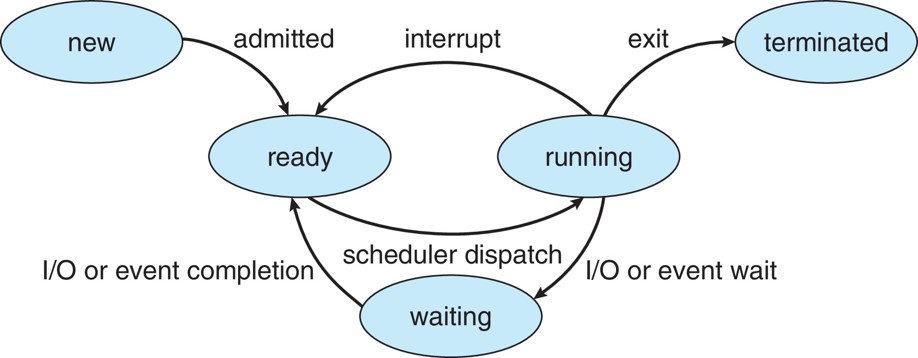
\includegraphics[width=0.6\linewidth]{fig/5-state-process-model.jpg}
	\end{figure}
	\item 优先级
	\item 程序计数器(PC)
	\item 内存指针:报错指向程序代码、相关数据和共享内存的指针
	\item 上下文数据(context):进程被中断时寄存器中的数据
	\item IO状态信息
	\item 记账信息(accounting):占用处理器时间、时钟数总和、时间限制等
\end{itemize}

% 如果想要进程之间交互,则通过文件进行,如sublime编辑文件,gcc对其进行编译

内存组织:代码段、数据段、堆段、栈段(从小地址往大地址)
\begin{figure}[H]
\centering
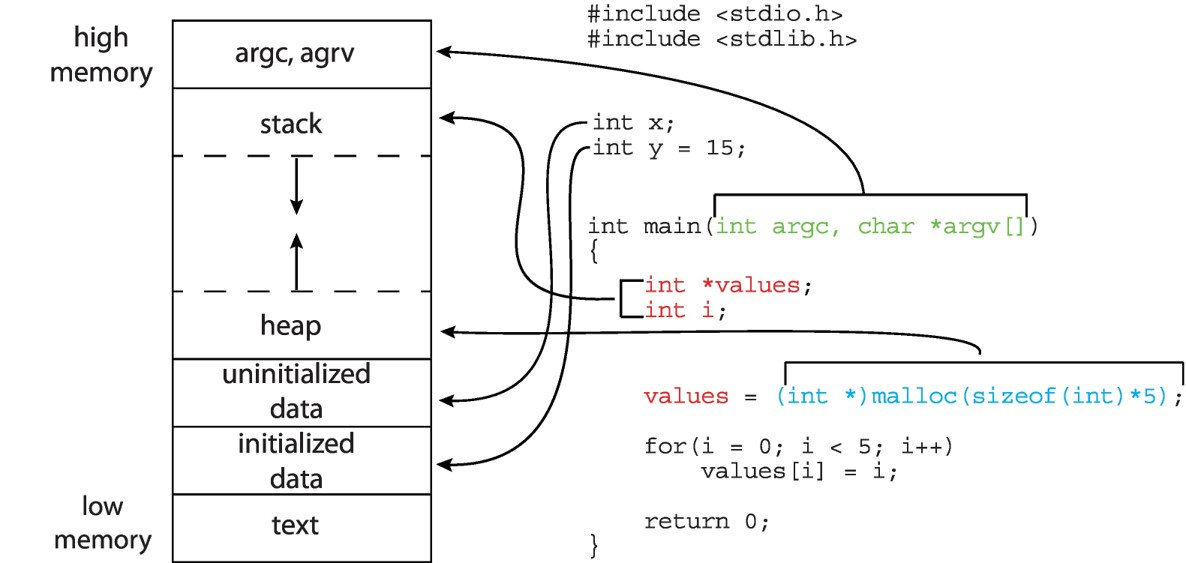
\includegraphics[width=0.8\linewidth]{fig/C_memory.jpg}
\end{figure}

可以参考原始的UNIX论文\footnote{\url{http://www.scs.stanford.edu/19wi-cs140/sched/readings/unix.pdf}}。
\begin{itemize}
	\item 创建进程:fork、waitpid
	\item 删除进程:exit、kill
	\item 执行进程:execve
\end{itemize}

进程切换:扔掉堆、数据段,读入新代码段、数据段,重设栈段、堆段,初始化寄存器,开始执行